\documentclass[sigconf]{acmart}
%%%% As of March 2017, [siggraph] is no longer used. Please use sigconf (above) for SIGGRAPH conferences.
\usepackage{tikz}
\usepackage{listings}
\usepackage{color}  % Optional for coloring code

% Configuration of code listings
\lstset{
  language=Java,                 % the language of the code
  basicstyle=\ttfamily\small,    % the size of the fonts used for the code
  numbers=left,                  % where to put the line-numbers; possible values are (none, left, right)
  numberstyle=\tiny\color{gray}, % the style of the line-numbers
  stepnumber=1,                  % the step between two line-numbers. If it's 1, each line will be numbered
  numbersep=5pt,                 % how far the line-numbers are from the code
  backgroundcolor=\color{white}, % choose the background color; you must add \usepackage{color}
  showspaces=false,              % show spaces adding particular underscores
  showstringspaces=false,        % underline spaces within strings only
  showtabs=false,                % show tabs within strings adding particular underscores
  frame=single,                  % adds a frame around the code
  rulecolor=\color{black},       % if not set, the frame-color may be changed on line-breaks within not-black text
  tabsize=2,                     % sets default tabsize to 2 spaces
  captionpos=b,                  % sets the caption-position to bottom
  breaklines=true,               % sets automatic line breaking
  breakatwhitespace=false,       % sets if automatic breaks should only happen at whitespace
  title=\lstname,                % show the filename of files included with \lstinputlisting; also try caption instead of title
  keywordstyle=\color{blue},     % keyword style
  commentstyle=\color{green},    % comment style
  stringstyle=\color{red},      
  escapeinside={\%*}{*)},        % if you want to add LaTeX within your code
  morekeywords={*,...}           % if you want to add more keywords to the set
}

%%%% Proceedings format for SIGPLAN conferences 
% \documentclass[sigplan, anonymous, review]{acmart}

%%%% Proceedings format for SIGCHI conferences
% \documentclass[sigchi, review]{acmart}

%%%% To use the SIGCHI extended abstract template, please visit
% https://www.overleaf.com/read/zzzfqvkmrfzn
\AtBeginDocument{%
  \providecommand\BibTeX{{%
    \normalfont B\kern-0.5em{\scshape i\kern-0.25em b}\kern-0.8em\TeX}}}

% \copyrightyear{2019}
% \acmYear{2019}
% \setcopyright{rightsretained}

%%
%% The majority of ACM publications use numbered citations and
%% references.  The command \citestyle{authoryear} switches to the
%% "author year" style.
%%
%% If you are preparing content for an event
%% sponsored by ACM SIGGRAPH, you must use the "author year" style of
%% citations and references.
%% Uncommenting
%% the next command will enable that style.
%%\citestyle{acmauthoryear}

%%
%% end of the preamble, start of the body of the document source.
\begin{document}

%%
%% The "title" command has an optional parameter,
%% allowing the author to define a "short title" to be used in page headers.
\title{Onion Router}

%%
%% The "author" command and its associated commands are used to define
%% the authors and their affiliations.
%% Of note is the shared affiliation of the first two authors, and the
%% "authornote" and "authornotemark" commands
%% used to denote shared contribution to the research.
\author{Ivan Krstev}
\email{89211055@student.upr.si}
\affiliation{%
  \institution{Famnit, University of Primorska}
  \city{Koper}
  \country{Slovenia}
}

% A clear and well-documented \LaTeX\ document is presented as an
%   article formatted for publication by ACM in a conference proceedings
%   or journal publication. Based on the ``acmart'' document class, this
%   article presents and explains many of the common variations, as well
%   as many of the formatting elements an author may use in the
%   preparation of the documentation of their work.


%%
%% The abstract is a short summary of the work to be presented in the
%% article.
\begin{abstract}
    This \LaTeX\ report document presents a Java-based implementation of the Tor network, aimed at enhancing HTTP request anonymity using Docker for containerization. The project demonstrates Java's capability to replicate essential features of the Tor network, focusing on secure, anonymous web communication and scalability. Key challenges addressed include secure data transmission, efficient routing, and system scalability within a Dockerized environment.
\end{abstract}

%%
%% The code below is generated by the tool at http://dl.acm.org/ccs.cfm.
%% Please copy and paste the code instead of the example below.
%%
\begin{CCSXML}
<ccs2012>
   <concept>
       <concept_id>10003033.10003083.10003014</concept_id>
       <concept_desc>Networks~Network security</concept_desc>
       <concept_significance>500</concept_significance>
       </concept>
   <concept>
       <concept_id>10003033.10003058.10003059</concept_id>
       <concept_desc>Networks~Intermediate nodes</concept_desc>
       <concept_significance>300</concept_significance>
       </concept>
   <concept>
       <concept_id>10003033.10003079.10011672</concept_id>
       <concept_desc>Networks~Network performance analysis</concept_desc>
       <concept_significance>100</concept_significance>
       </concept>
 </ccs2012>
\end{CCSXML}
\ccsdesc[500]{Networks~Network security}
\ccsdesc[300]{Networks~Intermediate nodes}
\ccsdesc[100]{Networks~Network performance analysis}

%%
%% Keywords. The author(s) should pick words that accurately describe
%% the work being presented. Separate the keywords with commas.
\keywords{Dark Web, Relays, Network Security, Anonymity, Privacy, Onion Routing}

%%
%% This command processes the author and affiliation and title
%% information and builds the first part of the formatted document.
\maketitle
\pagestyle{plain} % removes headers


\section{Introduction}
As internet usage permeates all facets of life, the importance of online anonymity has escalated. The Tor network, known for its ability to shield user identities through multi-node routing, exemplifies a critical tool for maintaining privacy and countering censorship. This project extends these concepts through a Java-based implementation focused on securely and anonymously handling HTTP requests—essential for private web browsing.

Java provides robust networking capabilities and cross-platform support, which are essential for this type of system. Docker is employed to virtualize network relays, facilitating testing and evaluation of the system under conditions that mimic real-world operation. This use of Docker ensures fast deployment and managing of relays while testing them for different purposes and highlighting a commitment to modern, efficient development practices and system reproducibility.

The project's goals are to replicate Tor’s anonymization functions, address network security programming challenges, and assess tor network replication in a Dockerized environment. This report will explore the development methods used, the architectural decisions, and the insights gained from implementing and testing the system.


\section{Background}

\subsection{Tor Network Basics}

The Tor network, or The Onion Router, is a distributed system designed for anonymous communication across the Internet. It achieves anonymity by directing Internet traffic through a worldwide volunteer overlay network consisting of thousands of relays. The process involves encrypting the data multiple times and sending it through a series of relays, each one decrypting a layer of encryption to reveal the next relay address in the circuit. This method is used to prevent anyone from knowing the complete path between the user and the destination website, effectively obscuring who is communicating with whom.

Key features of Tor include:
\begin{itemize}
    \item Onion Routing: Data packets are encrypted in layers—like an onion—and each node only peels away a single layer to reveal the next node's address.
    \item Circuit Establishment: A path through the network is randomly established at the start of each session, and all packets in the same session follow this path.
    \item End-to-End Encryption: Provides strong privacy protections by ensuring that data is readable only by the intended recipient.
\end{itemize}

\subsection{Related}

Previous research and implementations of Tor and some similar anonymizing technologies have primarily focused on enhancing privacy, reducing latency, and improving the scalability of the network. Notable contributions include:
\begin{itemize}
    \item Enhanced Tor Protocols: Modifications to the original Tor protocols to improve security against potential attacks and surveillance.
    \item Alternative Anonymity Systems: Development of other systems like I2P (Invisible Internet Project) and Freenet that also use similar concepts of decentralized routing and data encryption.
    \item Performance Studies: Extensive analyses have been conducted to understand the trade-offs between anonymity, latency, and throughput within these networks.
\end{itemize}


\section{System Design}

\subsection{Architecture Overview}
The system architecture for the Java-based Tor-like network is designed to emulate the key characteristics of the original Tor network, focusing on security, anonymity, and scalability. The design incorporates multiple nodes or relays, organized in a decentralized manner, through which encrypted HTTP requests are routed. The primary components of the architecture include:

\begin{itemize}
    \item Client Application: Initiates the connection, prepares HTTP requests, and handles responses. It also manages data encryption before sending it through the network.
    \item Entry Relay: The first point of contact in the network for encrypted data, which strips away the first layer of encryption and forwards the data to a middle relay.
    \item Middle Relays: Responsible for further peeling off layers of encryption and forwarding data toward the exit relay. These nodes increase the anonymity of the routing process.
    \item Exit Relay: The final relay that decrypts the last layer of encryption and forwards the original HTTP requests to the destination server.
    \item Tor Relays Directory Server: Maintains a list of active nodes in the network and their statuses, providing clients with up-to-date information about possible routes.
    \item Final Destination Server: Simulates the server that would typically receive and respond to requests in a real-world scenario. This component is essential for testing the network’s effectiveness in handling and delivering the requests securely and anonymously.
\end{itemize}

The system utilizes Docker containers to isolate each network component, enhancing security and replicability of the environment. Docker also facilitates scaling the number of relays based on demand without significant changes to the existing infrastructure, for further extending the onion router network.

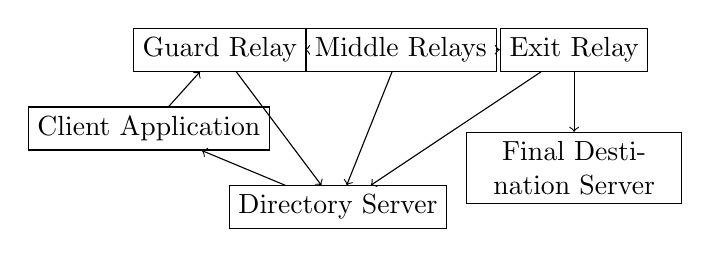
\begin{tikzpicture}
    \node (client) at (-0.4,-1) [draw, rectangle] {Client Application};
    \node (guard) at (0.5,0) [draw, rectangle] {Guard Relay};
    \node (middle) at (2.8,0) [draw, rectangle] {Middle Relays};
    \node (exit) at (5,-0) [draw, rectangle] {Exit Relay};
    \node (destination) at (5,-1.5) [draw, rectangle, text width=2.5cm, align=center] {Final Destination Server};
    \node (directory) at (2,-2) [draw, rectangle] {Directory Server};
    \draw[->] (client) -- (guard);
    \draw[->] (guard) -- (middle);
    \draw[->] (middle) -- (exit);
    \draw[->] (exit) -- (destination);
    \draw[->] (directory) -- (client);
    \draw[<-] (directory) -- (guard);
    \draw[<-] (directory) -- (middle);
    \draw[<-] (directory) -- (exit);
\end{tikzpicture}

\subsection{Component Details}
Each component is implemented in Java, leveraging its extensive network programming libraries and concurrency features to manage multiple simultaneous connections efficiently:

\begin{itemize}
    \item Encryption Module: Utilizes Java's cryptographic packages to handle the encryption and decryption processes. It ensures that each layer of encryption is independent and secure.
    \item Routing Algorithm: A custom algorithm is developed to select the path through the network dynamically based on real-time data on network congestion and node reliability.
    \item HTTP Handling: Specialized classes are designed to manage HTTP request packaging and unpacking, ensuring that all data remains intact and unaltered throughout the transmission process.
    \item Docker Configuration: Dockerfiles and Docker Compose scripts are used to define the setup for each type of relay and the directory server, ensuring that each container is configured with the necessary dependencies and runtime environment.
\end{itemize}


\section{Implementation}
\subsection{AES and RSA encryption/decryption}
In the secure communications setup of the Tor-like network, RSA and AES encryption technologies are used in conjunction to ensure robust security with efficient data handling.
Key features of combining RSA with AES:
\begin{itemize}
    \item RSA Encryption: Used primarily for encrypting the AES key. RSA is a public-key encryption algorithm that allows secure key exchange without the parties needing to share a secret key beforehand. However, due to its computational intensity, slow speed and limitations in data size (it can only encrypt data smaller than the key size), RSA isn't suited for encrypting large data payloads directly. The RSA methods use the RSA/ECB/OAEPWITHSHA-256ANDMGF1PADDING algorithm.
    \item AES Encryption: Used for encrypting the actual HTTP payload. AES is a symmetric key encryption algorithm, known for its speed and efficiency in encrypting large amounts of data. Once the AES key itself is securely encrypted with RSA, the AES key is then used to encrypt and decrypt substantial data payloads quickly and securely. The AES methods use the AES/GCM/NoPadding algorithm.
\end{itemize}

\begin{lstlisting}
// RSA.java - Encrypt AES key method
public static byte[] encryptKey(SecretKey aesKey, PublicKey publicKey) throws Exception {
    Cipher cipher = Cipher.getInstance("RSA");
    cipher.init(Cipher.ENCRYPT_MODE, publicKey);
    return cipher.doFinal(aesKey.getEncoded());
}
// AES.java - Decrypt method
public static String decrypt(byte[] cipherText, SecretKey key) throws Exception {
    Cipher cipher = Cipher.getInstance("AES");
    cipher.init(Cipher.DECRYPT_MODE, key);
    byte[] decryptedBytes = cipher.doFinal(cipherText);
    return new String(decryptedBytes);
}
\end{lstlisting}

\subsection{Client's HTTP Request Payload}
The HttpPayload class encapsulates the HTTP headers and body of a request. It is designed so that only the final exit relay has the ability to fully decrypt and understand the contents, ensuring that intermediate nodes cannot access or interpret the sensitive details of the HTTP communication.
\begin{lstlisting}
public class HttpPayload {
    private String method;
    private byte[] body;
    private Map<String, String> headers;

	// ... Constructors, getters and setters
}
\end{lstlisting}
\subsection{Relay Node Message Model}
The RelayNodeMessage class is designed for secure communication across the relay nodes. It is used to forward the encrypted AES key and the encrypted payload as JSON object to the next relays. It encapsulates encrypted messages and their corresponding AES keys, encrypted using RSA. Relay nodes decrypt the AES key with their private RSA key, then decrypt the message to obtain or forward the HttpPayload.
\begin{lstlisting}
public class RelayNodeMessage {
    private String encryptedMessage;
    private String encryptedAESKey;

    // ... Constructors, getters and setters
}
\end{lstlisting}


\subsection{Nodes Directory Server}
The TorNodesServer manages the network’s relay nodes, storing details in TorNodeInfo objects. It handles POST requests at the /add endpoint to add new relays, updating the network topology accordingly. Additionally, it processes GET requests at the /get-nodes endpoint to determine and select new paths for routing traffic, ensuring efficient and secure data transmission across the network

\begin{lstlisting}
public class TorNodeInfo {
    private String destination;
    private String publicKey;
    private String address;
    private RelayStatus relayStatus;

    // ... Constructors, getters and setters
}
\end{lstlisting}

The shuffle\_nodes method organizes a secure and randomized path through the Tor-like network by separating connected nodes into entry, middle, and exit categories. It ensures at least one entry and exit node are available, randomly selects these endpoints, and shuffles the middle nodes to construct a diverse route. The method then assembles these nodes into a path sequence from entry to exit, enhancing route unpredictability and security. For simplicity, only 8 nodes at most are selected always(1 entry, 6 middle, 1 exit).

\begin{lstlisting}[caption=The Routing Algorithm]
private List<TorNodeInfo> shuffleNodes() {
    List<TorNodeInfo> entryNodes = new ArrayList<>();
    List<TorNodeInfo> middleNodes = new ArrayList<>();
    List<TorNodeInfo> exitNodes = new ArrayList<>();
    Collections.shuffle(connectedNodes);
    for (TorNodeInfo node : connectedNodes)
        switch (node.getStatus()) {
            case ENTRY:
                entryNodes.add(node);
                break;
            case MIDDLE:
                middleNodes.add(node);
                break;
            case EXIT:
                exitNodes.add(node);
                break;
        }
    if (entryNodes.isEmpty() || exitNodes.isEmpty())
        return new ArrayList<>();
    Collections.shuffle(entryNodes);
    TorNodeInfo entryNode = entryNodes.get(0);
    TorNodeInfo lastExitNode = exitNodes.remove(exitNodes.size() - 1);
    middleNodes.addAll(exitNodes);
    Collections.shuffle(middleNodes);
    if (middleNodes.size() > 6)
        middleNodes = middleNodes.subList(0, 6);
    List<TorNodeInfo> shuffledNodes = new ArrayList<>();
    shuffledNodes.add(entryNode);
    shuffledNodes.addAll(middleNodes);
    shuffledNodes.add(lastExitNode);
    return shuffledNodes;
}
\end{lstlisting}

\subsection{The Relay Server}
\subsubsection{Relay Node Functionality Overview}
\begin{itemize}
    \item Initialization: The RelayNode initializes a server on a specified port(used the same for all routers) and configures itself based on the relay status (Entry, Middle, Exit) which receives through environment variable. It generates a public-private key pair for secure communication.
    \item Registration: Upon starting, it registers itself with the TorNodesServer by sending its public key, status, and address to the server using a POST request. This allows the network to track and utilize this node for routing traffic.
    \item Server Operation: Continuously listens for incoming HTTP requests, which are handled by RelayHandler.
\end{itemize}
\subsubsection{Relay Handler Overview}
\begin{itemize}
    \item Request Processing: This handler takes in HTTP requests, marks them as handled, and proceeds based on the encrypted content it receives.
    \item Decryption and Routing:
    \begin{itemize}
        \item The encrypted message is decrypted using the private key of the relay node.
        \item The decrypted payload determines whether the message should be forwarded to its final destination or to another relay node.
    \end{itemize}
    \item Forwarding:
        To Final Destination or Next Relay: The payload is universal for all relays. It is handled the same for forwarding to the next relay or the final destination
    \item Error Handling: Any exceptions during the forwarding process result in an internal server error response, maintaining the integrity of the network by not leaking details about the failure.
    \item Dynamic HTTP Methods: The method to contact the final destination dynamically adapts based on the HttpPayload (GET, POST, PUT, DELETE), ensuring compatibility with various types of HTTP interactions.
\end{itemize}
\begin{lstlisting}[caption=The Routing Algorithm]
@Override
public void handle(String target, Request baseRequest, HttpServletRequest request, HttpServletResponse response)
        throws IOException {
    baseRequest.setHandled(true);
    try {
        System.out.println("Received request from: " + request.getRemoteAddr() + ":" + request.getRemotePort());

        RelayNodeMessage relayNodeMessage = objectMapper.readValue(request.getInputStream(), RelayNodeMessage.class);
        HttpPayload decryptedPayload = relayNodeMessage.decryptAndDeserializeEncryptedMessage(privateKey);
        
        byte[] decodedBytes = Base64.getDecoder().decode(decryptedPayload.getBody());
        String bla = new String(decodedBytes, StandardCharsets.UTF_8);
        decryptedPayload.setBody(bla);
        byte[] forwardResponse = forwardRequestToFinalDestination(decryptedPayload);
        System.out.println("Received response from the final destination: " + new String(forwardResponse));
        response.setStatus(HttpServletResponse.SC_OK);
        response.setContentType("application/json");
        response.getOutputStream().write(forwardResponse);
    } catch (Exception e) {
        response.setStatus(HttpServletResponse.SC_INTERNAL_SERVER_ERROR);
        response.getWriter().println("Internal Server Error");
    }
}
\end{lstlisting}

\subsection{Tor Client}
The TorClient essentially packages and sends user data through a secure, anonymized channel, employing RSA for AES key encryption and AES for subsequent message encryption(the http payload), following the principles of onion routing:
\begin{itemize}
    \item Retrieves Tor Nodes: Fetches a list of active Tor nodes from the server to determine the routing path for the outgoing request.
    \item Encrypts the Message: Sequentially encrypts the HTTP payload along modifying it for forwarding the requests from relay to relay, till the exit node where the original HTTP payload is discovered.
    \item Routes the Request: It sends the encrypted message through the network, starting from the last node to the first, ensuring each message is only decryptable by its intended next-hop using layered encryption (onion routing).
    \item Communicates with the entry relay: Uses the HttpMessage-Dispatcher to handle the communication between the client and the entry relay.
\end{itemize}
\begin{lstlisting}[caption=Tor Client Request Sending]
public void sendRequest(HttpPayload httpPayload) throws Exception {
    TorNodeInfo[] torNodes = getTorNodesFromServer();
    if (torNodes == null || torNodes.length == 0) return;
    String destination = torNodes[0].getAddress(); // First (entry) relay node address
    for (int i = torNodes.length - 1; i >= 0; i--) {
        if (i != torNodes.length - 1) {
            httpPayload.setDestination(torNodes[i + 1].getAddress());
            httpPayload.setMethod("POST");
            Map<String, String> headers = new HashMap<>();
            headers.put("Content-Type", "application/json");
            httpPayload.setHeaders(headers);
        }
        String httpPayloadSerialized = objectMapper.writeValueAsString(httpPayload);
        SecretKey AESKey = AES.generateKey();
        String encryptedPayloadJSONString = AES.encrypt(httpPayloadSerialized, AESKey);
        RelayNodeMessage relayNodeMessage = new RelayNodeMessage(encryptedPayloadJSONString, RSA.encrypt(AESKey, torNodes[i].parseAndGetPublicKey()));
        httpPayload.setBody(objectMapper.writeValueAsString(relayNodeMessage));
    }
    System.out.println("Response from tor client: " + new HttpMessageDispatcher().sendPostRequest(destination, new String(httpPayload.getBody())));
}
\end{lstlisting}

\subsection{Message Receiver}
The MessageReceiver Java class is designed to act as the final destination within a Tor-like network, simulating the endpoint for messages sent through the network. It features a server setup using Jetty, configured to listen on all network interfaces at port 8080. The server employs a MessageReceiver Servlet to handle HTTP requests of various types—POST, GET, PUT, and DELETE.

Key Functionalities Include:
\begin{itemize}
    \item HTTP Request Handling: The servlet processes incoming HTTP requests, echoing specific responses based on the request type. This allows it to simulate how a real server might respond to different actions.
    \item Request Logging: It captures and logs details about each request, including headers and the body content, providing visibility into the data transmitted through the network.
    \item Dynamic Responses: Depending on the method invoked (POST, GET, PUT, DELETE), it responds with a playful message, acknowledging the received action in a straightforward manner.
\end{itemize}
\begin{lstlisting}[caption=Final Destination Server]
@Override
protected void doPost(HttpServletRequest req, HttpServletResponse resp) throws IOException {
    System.out.println("MessageReceiver: POST Request received!");
    System.out.println("Request headers:");
    printHeaders(req);
    // Read and log the request body
    String requestBody = getRequestBody(req);
    System.out.println("Request body: " + requestBody);
    // Sending response back to the client
    resp.setContentType("text/plain");
    resp.getWriter().println("Created something new xD!");
}

@Override
protected void doGet(HttpServletRequest req, HttpServletResponse resp) throws IOException {
    System.out.println("MessageReceiver: GET Request received!");
    System.out.println("Request headers:");
    printHeaders(req);
    // Sending response back to the client
    resp.setContentType("text/plain");
    resp.getWriter().println("Got something new xD!");
}
// ... Similar handlers for PUT and DELETE requests
\end{lstlisting}

\subsection{Sender}
The Sender class initiates the sending process within the tor network. It waits for a brief period(due to servers turning on in Docker), then constructs and sends an HTTP request using the TorClient instance, specifying the destination address, request method, message content, and optional headers. This class serves as a simple interface for sending requests securely through the network.

\section{Testing and Results}
\subsection{Performance Evaluation}
Latency Measurements: They revealed that delays introduced by encryption, routing, and decryption were relatively low. However, further configuration adjustments could potentially reduce these latencies even more. Optimizing relay node efficiency and improving data routing strategies are key areas for enhancing speed without compromising the network's security, making it more suitable for time-sensitive applications.
\subsection{Results}
\begin{itemize}
    \item Functionality: All components operated as expected, with messages being correctly encrypted, routed, and decrypted.
    \item Security: No vulnerabilities were exposed during the testing, confirming the robustness of the encryption and the anonymity provided by the routing protocol.
    \item Performance: The network maintained functionality under stress conditions and managed to handle expected loads with acceptable latency and throughput rates(considering the whole virtual network is on one host only).
\end{itemize}


\section{Comparisons to Real-Life}
In real-life case scenario, every condition will have to be considered differently, not like the Docker virtualization of the tor network. The performance and security will be affected my more factors like the geo-location of the relays, their statuses, their networks and their load balancing.


\section{Conclusion and Future Work}
This project successfully demonstrates the capabilities of a Java-based implementation of a Tor-like network, achieving secure and anonymous routing of HTTP requests. Throughout testing with Docker, the system maintained the standards of data confidentiality and integrity, showcasing its potential for real-world applications where privacy and security are paramount.

However, one limitation of the current implementation is that it does not incorporate padding to maintain a consistent message size. Without padding, the messages could potentially reveal patterns or metadata about the traffic, slightly weakening the anonymity guarantees of the network.

\begin{itemize}
    \item Padding Issue: Future enhancements could explore implementing standardized padding mechanisms like PKCS\#7, or by adding a custom padding of missing bytes to the payload body. Experimenting with different padding lengths and types will help in normalizing the message sizes.
    \item Performance Optimization: Further reduce latency and increase throughput through advanced load-balancing algorithms and network topology optimization.
    \item Scalability Enhancements: Develop dynamic scaling solutions to manage more relay nodes efficiently as network traffic increases.
    \item Security Upgrades: Continuously update encryption algorithms and protocols, including adopting quantum-resistant methods to safeguard against evolving cyber threats.
    \item User Authentication and Access Control: Implement sophisticated authentication and access control mechanisms to enhance security and user management.
    \item Automated Error Handling and Self-Recovery: Increase network reliability with automatic failure detection and recovery mechanisms to minimize downtime.
    \item Comprehensive Data Analytics: Utilize analytics to gain insights into network traffic, node performance, and security, guiding future optimizations.
\end{itemize}

\section{Appendix: Source Code}
The full source code and documentation for all implementations described in this report are available in the following GitHub repository: \url{https://github.com/ivankrstev/OnionRouter}

\end{document}
